\chapter{因缘}

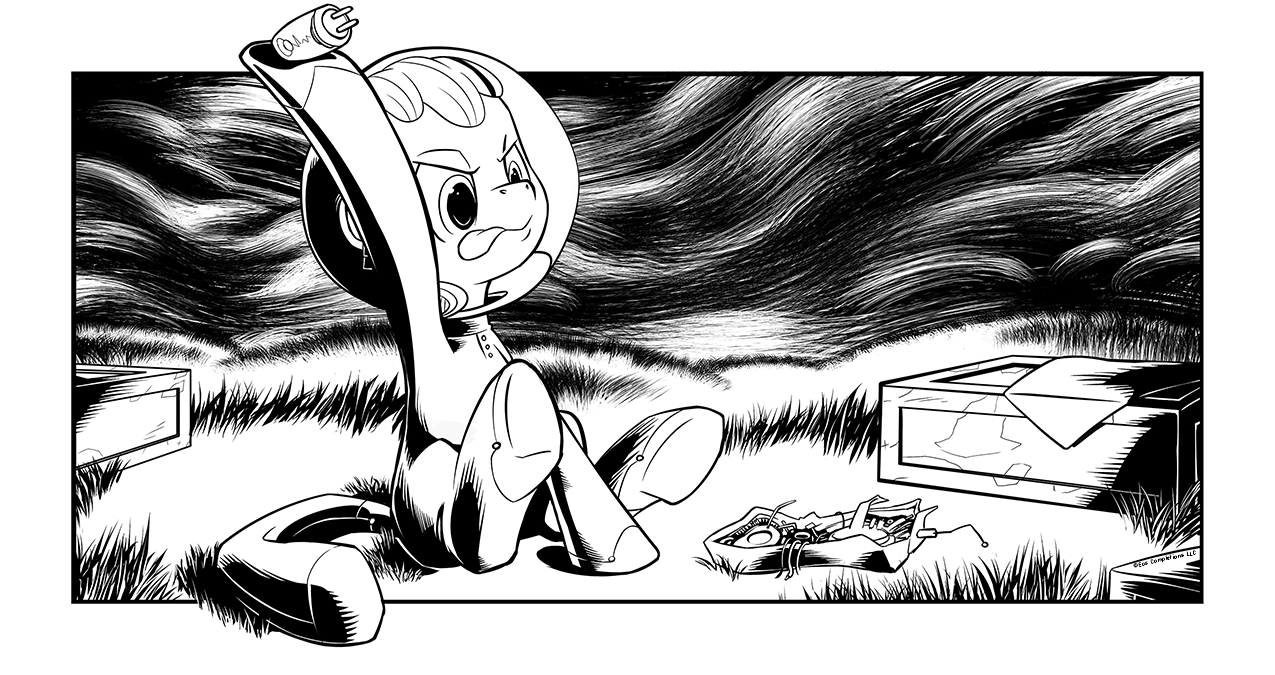
\includegraphics[width=0.9\linewidth]{image17.png}

\begin{intro}
    整个世界都在问这个问题:
    
    {\heiti 谁才是坏蛋?}
\end{intro}

\daytimeplace{13}{6:45 PM}{纪念碑镇北部,52号国道南段}{The Memorial northern picnic area, Big 52 S Branch}

一个雌驹和一个公马顺着52国道南下,他们都背着突击步枪,雌驹穿着保安的防弹衣,而她的伙伴则穿着一身由各种金属板焊在一起的奇怪铠甲,看起来就像是某种廉价喜剧里面的外星马一样。

% FIXME: 译文错误

「我们到底是为了啥离开隧道镇,明明糖霜山的要塞易守难……嗷!」

快乐扳机照坏枪的脑门上就是一蹄子,「我们蹲在要塞,然后看着野牛帮在52国道六成的领土上肆虐么!你怎么是这么一个自私的傻蛋!」

公马撇开视线,「我才不自私……我只是……担心你而已。我不想让你像这样冒险。」雌驹白了他一眼,公马识趣的闭嘴了,不过这也只能让这个热恋中的傻瓜安静半分钟,「至少我们现在先停下过夜吧,纪念碑镇就在附近了。」

「好吧,懒蛋,随你!天啊,你知道你有多烦吗?」快乐扳机咆哮着,「DJ好货已经说了那个镇已经被遗弃了,我觉得那里至少会有比帐篷更好的休息地方。」

说到这里,那座远处倒下的小马国雕像被几个出现的黑影挡住了。

\horizonline

\daytimeplace{13}{7:00 PM}{纪念碑南部公园,52号国道南段}{The Memorial southern picnic area, Big 52 S Branch}

在头盔完全修复之后,一个闪烁的粉色亮点出现在显示屏中央。

「{\mt 系统重启完毕。所有功能正常。自检开始。目标:001号,快乐帕比,雌性陆马幼驹。目标已死亡,体征一切正常。自检完毕。}」

帕比慢慢地睁开眼睛,还是有点昏昏沉沉的。至少从她醒来的地方判断,唉,果然没有从噩梦里面醒来。四周还是枯黄的草和死去的树木,不是她自己的房间。小雌驹叹着气,继续检查粉色箭头的方向,不过某些东西引起了她的注意。

「声音先生,那是啥啊?」

「{\mt 分析中……坦克残骸。威胁等级:无。}」

「不是说那坏机器,傻声音!」帕比叹了口气走到那个东西旁边,「是这个闪光的东西。」

「{\mt 分析中,短波电台,获取加密频道中,新增加通信频道,接到呼叫。}」

「耶!电话!让我接,我要接电话!我超喜欢接电话,拜托了!」帕比清了清嗓子,「嗯哼!您好,漂漂马,妈妈现在不在家!」

一个又惊又怒的雌驹声音从听筒里面传来,「你丫是哪根葱?好运姐在哪?」

耶!是猜谜游戏!「嗨,我是快乐帕比!谁是好运姐?我知道有个小马叫好运气,可以么?」

对方把电话粗暴地挂断了,帕比呆呆地说:「唉,又是恶作剧电话,好吧,别生气,否则正中他们下怀。」帕比耸了耸肩继续前进。

「{\mt 注意:新呼叫,打开通信频道。}」

帕比还没时间回答,和刚才相同的那个声音又出现了。

「听好了混蛋,我觉得这个频道现在不安全了,不过老板现在已经火大了,如果你们丫的不赶紧把坦克开回来那你们就有大麻烦了,懂了么好运,我再说一次,跟灰质那傻叉说叫他麻溜地把坦克开回来,这是老娘最后一次……」

「呦呵,漂漂马又说不明觉厉的话了。」帕比咯咯笑着,作为一个恶作剧电话的话这个蛮有趣的。

「我肏……怎么又是你?肏你妈!」通讯又一次被切断了。

帕比歪着头:「好奇怪哦,或许我们应该赶紧走?」

「{\mt 肯定,主目标地点不在这个方位,注意:新呼叫,打开通信频道。}」

同样的声音再一次说话了,「好运姐,好运姐,这里是小马要塞,请回答。」

帕比笑着回话:「不是,又是我!没关系么?」

那个神秘的声音叹了口气放弃了,「听好,小鬼,我不知道为啥又是你,不过我现在要和某马对话,而你的无线电一直干扰我们的通讯,你到底从哪儿得到这个频道的频率和密码的?」

「什么?密码?我知道!密码是快乐帕比!」小雌驹回答。

「死熊孩子!给老娘关了你的无线电!我正忙着联系一群酒驾坦克手,除非你看过一个坦克在附近晃悠,要不然就别添乱。」

帕比戳着头盔,认真的想着,「坦克?那东西长什么样?」

「你……你有完没完?好吧,那东西很大,有个炮塔有个大炮,还有履带……」声音顿了一下又说:「你见过么?」

帕比看了看就在她旁边冒烟的残骸,然后回答:「呃……那东西是不是还会嘣嘣嘣地把炸弹到处丢?」

「对对对!你见过么?」

「嗯哼,」帕比点了点头,「那是个大坏蛋,所以我用石头把它砸爆了!」

然后一阵长长的沉默之后,对面大发雷霆,「真他妈的,你为啥不找个仙人掌自个儿撞死去?」然后通讯又被切断了。

帕比耸了耸肩,这个新的声音很奇怪,不过帕比应该跟着箭头走,没时间再接恶作剧电话了,不过……她是不是应该对那个恶作剧电话的马来个恶作剧电话?

「呃,声音先生,你能呼叫小马要塞么,超超拜托!」

「{\mt 肯定,打开通讯频道。}」

那个雌性的声音立刻说:「这里是小马要塞,听到请讲!」

「啊……嘻嘻……我是……嘻嘻……咸蛋,请找……嘻嘻……笨蛋先生……嘻嘻……」帕比一边咯咯笑着一边说,她在漫画里面看过这个恶作剧,她自己一直想试试看。

% NOTE: ignore overfull

对面沉默了好久,最后小马要塞回答说:「你丫居然给老娘打恶作剧电话?等我告诉这个笨蛋先生,然后让他把你的屁股打开花。」

帕比大吃一惊:「不要!不要!拜托了,我很抱歉!别……别打我屁股!我会乖乖的!」

一阵大笑之后,那声音回答:「太迟了,恶作剧小鬼!看好你的屁股,因为咸蛋先生和笨蛋先生已经找你去了。」

「咿……呀!」

小雌驹撒开蹄子飞奔向山丘,就好像有无数打屁股板子追在后面一样。快跑吧黄色小鬼,快跑!

\horizonline

\daytimeplace{13}{7:30 PM}{纪念碑镇北部,52号国道南段}{The Memorial northern picnic area, Big 52 S Branch}

别飞得太高,也别飞得太低,老天马,不要一时冲动做傻事……

孤狼飞过重重山丘,寻找着远处可辨的地标,在过了花椰菜镇之后他一直保持低空滑翔,不过随着天色变暗地面上什么都看不清了。

「见鬼,我还是赶紧找个地方过夜,我可不想一头撞上强盗的巡逻队。」天马想着,落在一个小山丘上休息自己的翅膀,「好吧,我到哪了?」

DJ 一直用自己的哔哔小马用低音量播放着52电台,当音乐声停止DJ好货开始说话的时候他放下了地图仔细听着新闻。

「{\rt 好了,小马们,这里是DJ好货为您播报的52电台,不过现在没什么好消息。}」

DJ 叹了口气,听起来马上要哭出来的样子。

「{\rt 铁砧镇已经不复存在了,我前几分钟之前刚刚收到消息,野牛帮已经攻破城镇大门,幸存者撤退回了小镇的避难厩。野牛帮有重武器,战斗机器马,还有更多的东西……现在与一场血腥屠戮只有一道避难厩大门之隔的,是两百只小马,大多数都是妇孺。}」

孤狼叹了口气,摇着头小声说:「孩子,这可帮不上什么忙,在广播里面像个孩子一样哭鼻子不能解决问题,小马需要你的声音领导他们,而不是……」天马叹了口气,「难道每件事都非得我自己来才行?」

「{\rt 很抱歉,大家,我还不习惯做这个……不管怎么说这不是我的错,不过我认为我们还有希望,毕竟幸存者们固守的那扇避难厩大门不是那么容易打开的。所以,你们仔细想想,野牛帮的下一个受害者可能就是你,虽然你现在安全地缩在角落里面,但是你躲得了一时躲不了一世,52号国道是一个整体,如果铁砧今天陷落了,明天将会是花椰菜,然后是铁锈庄园……这样下去野牛帮的肆虐将不可阻挡。}」

孤狼打了一个响鼻收起了翅膀,静静听着那个雌驹的声音,DJ好货的语气也变得越来越自信,好像是她终于找到了她的信念。

「{\rt 但是!如果我们在那之前站在一起面对他们,如果我们能一起去拯救铁砧镇的那些无辜小马,我想我们还有胜算,只需要肩并肩,蹄挨蹄站在一起。孤狼已经去和你们一同战斗,我们只要追随他的脚步!}」

「还不赖,虽然还有很大进步空间,不过至少她没让他们能跑多远跑多远……」天马叹了口气,「至少证明把她留下不是错。」

「{\rt 我想我说得太多了,我们还是继续之前的音乐,这里为铁砧镇献上一曲,请不要轻易放弃,救援马上就到!坚持住小马们!我们只要相互信任,一切都会变好!}」


\begin{music}
    如果只有一匹马相信你
    
\begin{englishlyric}
    If just one pony believes in you,
\end{englishlyric}
    
    \medskip

    他强壮而又有力,深信着你
    
\begin{englishlyric}
    Deep enough and strong enough, believes in you,
\end{englishlyric}
    
    \medskip

    他忠贞而又强大,深爱着你
    
\begin{englishlyric}
    Hard enough and long enough, before you knew it,
\end{englishlyric}
    
    \medskip

    如果有那么一匹马,那么我也可以做到
    
\begin{englishlyric}
    Somepony would think, if he can do it, I can do it,
\end{englishlyric}
    
    \medskip

    我们大家都站在你那边
    
\begin{englishlyric}
    Making it two,
\end{englishlyric}
    
    \medskip

    你绝对不会孤独
    
\begin{englishlyric}
    Two whole ponies believe in you.
\end{englishlyric}
\end{music}

孤狼打了一个响鼻,「还真选了个不错的歌,虽然有点孩子气,不过既然我们是去拯救孩子们,那么我想这样也可以。」小马笑着,走向纪念碑镇。

\horizonline

\daytimeplace{13}{9:00 PM}{废土,52号国道南段}{Wastelands, Big 52 S Branch}

五个强盗现在完全摸不着头脑,因为站在他们面前的黄色幼驹违反了两条废土准则——首先小马们见到他们应该是掉头就跑,而不是跑过来求助。其次小马在连中数枪之后应该死掉,而不是像这个一样活蹦乱跳。

「求求求求求您了!快把我藏起来!他马上就追过来了,拜托,拜托!拜托了!」帕比焦急地来回踏着蹄子。「我已经说我很抱歉了,但是他还是要追我!」

一个脖子上留着一道大伤疤的陆马雄驹走向幼驹,而其他四个则举枪跟在后面,「你丫到底是谁,你丫到底是啥,什么东西能追你?而且为啥肏他妈的你还活着?」那马低头看着帕比胸口上的弹孔现在早已经消失了,而且她一点痛苦的表情都没有。所以说,听这个诡异的小孩把话说完是个好主意。

「呃……我……我是……」帕比愣住了,如果这些马其中之一是笨蛋先生或者咸蛋先生呢?她要放聪明点。「我……我是……啊……幽灵!我绝对是那个收音机里面一直在说的幽灵!而且,我的名字是……呃……不叫快乐帕比。」来回打量这几个小马之后,幼驹又弱弱地追问一句:「这里没有马叫笨蛋或者咸蛋吧?」

公马慢慢地点了点头,粉色的闪光双眸,黄色的防辐射服,不怕子弹……没错,就和那个传说中的幽灵一样,「所以……你就是52号国道的幽灵?」

「没错!」帕比点点头,现在她的说谎技巧就面临考验了。帕比,你要聪明点,露出不在乎的表情!

「你的名字是……『不叫快乐帕比』?」

「对对对!」看起来有效了!他们上当了!欢呼吧帕比,你是说谎话大师!

「那个52号国道的幽灵?那个拯救城市的机器马杀手?」除了第一位小马之外,其他几个都吓得退了一步。

「就是我!」帕比用力点着头。

「你想要我们的帮助?」公马有点迷糊了。

「没错!呃……如果说你们没有马叫笨蛋先生的话。」

「我……好吧,我叫砍刀,那个独角兽是伤管,他的娘们儿是切纸。然后那俩是臭尾和塑料花。」公马指着剩下的俩雌驹介绍着,除了伤管和切纸,其他两个都是陆马。

帕比松了一口气,「哎呦,真是太悬了,那啥,有个疯子正在追我,因为我给她打了一个恶作剧电话,所以她现在想打我屁股,我……我能……我能和你们混一会儿么?等他来的时候你们可以跟他说我是个好孩子让他不要打我屁股好么?超超拜托!」

砍刀看了看他缩在后面的伙伴,另外一个公马耸了耸肩,其他三个雌驹也一副不想管闲事的表情。「你真的只是因为有马想要打你屁股才跑的?」

小雌驹点点头。

强盗叹了口气,「你傻啊!」

「呃……或许有点?如果我真傻你们可以帮我么?」

公马又叹了口气,他今天叹了好多次气了,「反正你也会跟着我们,是吧?」

帕比笑着点了点头。

\horizonline

\daytimeplace{13}{10:00 PM}{纪念碑镇,52号国道南段}{The Memorial, Big 52 S Branch}

白先生一边把一个铁罐子塞进自己包包,一边冷笑着。「只是因为一个你不认识的小马,你就丢下自己的电台一路飞到这里?」

「差不多……我感觉到起风了,而且……我想要在那事情发生的时候在现场,我很惊讶你们也在这里……」孤狼看着窝棚里面的一群马回答着。

到目前为止,这里有一个来自沙漠里的先知,隧道镇的警长和她的……情夫?男友?都差不多,还有小马国最著名的盗墓者融金,还有这位白苹果家族的白先生和他侄子。

「你们有啥高见?」天马看着夜空等着先知开口。

「我们还在等其他朋友,我们明天再行动,现在野火正旺,我们必须等待火焰即将熄灭的时候再行动。」长耳闭上眼睛深吸一口气说。

「听好了,我才不管你那什么破预言!」快乐扳机打断她:「我只想知道帕比是否安全,你这个嗑药的知道么?」

独角兽雌驹睁开眼睛回答道:「我怎么可能知道,我不可能选择预知梦的内容。」

乐乐懒得理她,转头走向角落的那个尸鬼,融金在她来这里之后一句话也没说,不过他现在看起来心事重重。

「老木乃伊,你经常来北边……」雌驹对宝物猎手微微一笑,虽然不喜欢这个老尸鬼,不过他也没做什么惹雌驹厌恶的事情——至少现在还没。「我很好奇,那个幼驹对你做了什么?」

尸鬼转头看着这位守卫队长,「那个幼驹没有对我做什么……而是因为我没有对她做我该做的事情。」融金一声自嘲地冷笑就像是白骨刮过金属一般,「两个世纪以来,我第一次感觉到内疚,你相信么?」

灌木摇了摇头,现在这里看起来就像是那种「讲自己的故事」然后大家一起「哦,好可怜」叹息的社区集会。「你还是说吧,我觉得这里的大多数都活不下来,所以不必担心你的小秘密被别的马知道。」狙击手轻蔑地哼了一声,然后补充道:「等大家都讲完伤心事之后我们可以来场枕头大战了。」

白先生以蹄覆面,「灌木,你不说话没马当你是哑巴。」

尸鬼开始用他那沙哑的声音讲述自己的故事。

「我正好认识帕比的妈妈,阴雨。她也算是某种英雄,不过并不是那么特别,但是在炸弹刚刚落下来的那些日子里,每匹马都惶惶不可终日。是她组织起难民营,将我们聚集起来,给我们活下去的信念和力量,帮助了很多小马。她教会小马们如何自救,如何保护自己,然后又离开,去下一个城市,做同样的事情,在这片废土上点燃52国道沿途的文明之火。」

坏枪跳了起来,「既然你知道这些,你又和帕比说了什么?」

融金瞪着那个卫兵,低声说:「我能和她说什么?『抱歉你妈妈已经死了?』你有看过她的那双眼睛么?所以我送她去了象牙塔,希望那里的铁骑卫可以找到办法帮助她……」尸鬼顿了一下,然后又转开头补充道,「……安息。」

大家一瞬间都安静了下来,不过这时候快乐扳机叫了起来:「我说,象牙塔完全被毁了,你还送那孩子去那里?」雌驹怒气冲冲地举起枪,「你这个龟儿……」

坏枪和孤狼一起按下了女警卫,「乐乐,冷静,之后还有人在花椰菜看到了她,她没事的!」

融金叹了口气摇着头说:「没错,她肯定不会有事,而且有趣的是,象牙塔的大多数小马都安然无恙……不过是他们的老窝被炸了而已。如果有谁告诉我是那个孩子干的,我倒是一点都不奇怪。」

孤狼放开了快乐扳机,然后站起来说:「有两个被帕比救了的奴隶和我说,她看起来就和幽灵一样,子弹穿过她的身体就像什么也不存在一样,而她发着粉光的眼神催眠那些强盗自相残杀……话说,你们相信幽灵么?」

「我勒个去,」乐乐生气地大叫起来,「蠢蛋,别跟我说这个好么。我家那二货已经在通道镇问过这个问题了,虽然我承认这个幼驹看起来不太寻常,但是我亲自抱过她,我很确信她是真实存在的!」

白先生看着窗外说:「我觉得我们是不是至少有个放哨的,有几个小马从北边来了。」

所有的小马都转向长耳等她开口,先知微笑着站起来走向门口,「他们来的比预期的要早……我们去见见著名的铁骑卫吧。」

\horizonline

\daytimeplace{13}{10:30 PM}{废土,52号国道南段}{Wastelands, Big 52 S Branch}

小小的营火在营地中央跳跃着,两个陆马雌驹在煮着罐头装的食物,其他小马则在擦拭着武器,所有小马都尽量忽略帕比。

臭尾低声和伤管咬着耳朵,「你觉得他们已经打开避难厩了么?」

独角兽耸耸肩,继续擦拭着武器,「早晚的事,那些肥猪让我们饿了这么久,这次要把他们都宰了!」他啐了一口恶狠狠地说:「去年我们饿死了十一个,我现在已经等不及要杀进去让他们血债血偿了。」

塑料花冷笑着补充道:「那些肏蛋货占着所有肥沃田地,把所有好东西都自己独吞了……这次他们都要吐出来。」

砍刀也点了点头,「铁砧镇,铁锈庄园,盐块城,所有这些城市都要烧成灰烬!」

帕比虽然不太懂他们在说什么,不过她觉得他们清理武器的办法太没有效率了,有更好的办法把东西弄干净。「呃,为什么你们只是擦那当当响的东西,为什么不把那东西丢进水里洗,那多方便!」

一路上这个小雌驹绝对是有型的噪音源,无尽的语言折磨,那些强盗骂她也好,用枪打她也好,完全不管用,她就是在吧啦吧啦地说着,只有说要打她屁股还有点用处,不过没有马敢去碰这个完全不怕子弹的东西,而且从她身上弹孔里面漏出来的粉色烟雾看起来很危险,而且更恐怖的是,那些粉色烟雾就像有生命一样。

「这些枪要上油,除非你想它卡壳然后在你嘴里爆炸,」切纸解释道,「你根本不知道什么叫维修保养对吧?」

「维修?我当然会维修!我是最厉害的修理工!」

「修理工?你为啥不先修好自己的脑子。」雌驹笑了起来。

「不,我会修收音机,而且……而且我修了一个大电视!还让我的声音朋友动了起来,他超开心,嗯,我是个声音修理工,大概?」

切纸停下了活看着她,「你……真的会修电子设备?」

这是个好机会!帕比心想,如果让这些小马知道自己有多厉害,那么一定会和他们成为好朋友的!或许笨蛋先生来打她屁股的时候这些朋友可以帮她,或许这些朋友可以帮她找到妈妈!

「当然,我什么都修得好!」

独角兽飘着一个无线电台到帕比面前。「那你证明给我看,这东西下午就坏了,然后我们就和基地联络不上了,如果你能修好它我们就让你加入野牛帮。」

黄色小雌驹看着小无线电咯咯笑着:「上次我修好的那一台有一个屋子那么大呢!小菜一碟!」

咣!咣!咣!

帕比把无线电用力在地上摔着一直到它外壳裂开,然后她看了看里面,一副胸有成竹的样子,「嗯,我知道故障原因了,它坏了!」

独角兽以蹄覆面,正准备拿回比之前还坏得更彻底的无线电时,帕比拦住了她。

「现在我只要把一些闪闪发光的东西塞进去……」帕比拿出一个火花电池塞进可怜的收音机,然后用力敲打了几次,然后在一阵滋滋声中,无线电台恢复工作了。

「什么!你居然修好了?」雌驹一把从幼驹蹄子上抢过无线电,立刻联系基地,「红蟑螂呼叫小马要塞,请回答,重复一遍,红蟑螂呼叫小马要塞,请回答!」

所有小马都屏住呼吸静静的等待着回复。然后这个通信设备新的闪闪电池冒出一阵火花,随之发出一个声音:「这里是小马要塞,红蟑螂你们都去哪儿了?再不回来我们就把你们的东西拍卖了!」

随着这一句话,所有强盗都欢呼起来,兴奋的朝天开枪,帕比也咯咯笑着看着这一幕,砍刀走到她身边拍着她的头盔说:「干得好小家伙!谁知道你居然是个电子天才?我们完全误解你了,欢迎加入野牛帮!」虽然他还想说什么,不过切纸打断了他的话。

「灰质开着坦克不知到哪儿去了,老大想让我们赶紧回铁砧镇。」

塑料花摇着头,「那些傻货开着坦克跑了?我早和老大说过别给那群疯子那玩意,他们从来没想过野牛帮什么事情,他们只是想在52号国道上烧杀抢掠而已。」

「唉,随便了,」臭尾说,「反正我们还有坦克,而且还有机器马,我们这一次绝对不可战胜!」

伤管拍着帕比的背说:「小幽灵,想看看我们的基地么?」

「呃……我不知道……我应该去找我妈妈……她大概在那边……」帕比指着南方。

「那真是太好了!我们也去那边!」砍刀拍着幼驹的头盔,大家都在逗着小帕比玩,而帕比也觉得很开心。

这队强盗的领队说:「好了大伙,拔营,我们连夜赶回铁砧镇!」

\horizonline

\daytimeplace{13}{11:00 PM}{纪念碑镇,52号国道南段}{The Memorial, Big 52 S Branch}

诘责喝着他的茶,看着房间外面的窝棚,「很好,我们现在有个DJ,有个尸鬼,有个投机倒把的,有个瘾君子还有仨民兵?」

老书记官摇了摇头。

「52号国道的最后防线就是你们了?聘蹄的佣兵呢?」

冷浴耸了耸肩,不穿动力装甲的她看起来比一个孩子大不了多少。「随便了,反正我们也没期待它们,我们有自己的部队。」

「这些就是我们阿杰铁卫想要保护的小马么?」

帕拉丁皱着眉头看着诘责,「我可没有看到什么老弱病残,在我看来,他们不过是一群自发组织的民兵队而已,如果他们想参战,我不会阻止他们上前线,不过……」敲门声打断了她的话。

「请进。」

白先生推开门走了进来,「晚上好,书记官诘责和帕拉丁冷浴,」独角兽打量了它们一会然后说,「情况一切正常么?」

诘责打量着他说:「呦,52国道上最有权势的马来了,我可以问一下你,为什么只带了一个士兵来?或者……你们的其他后备队还在路上?」

老白摇了摇头:「不,我现在既不是白苹果的领袖也不是聘蹄的老大,我只是代表自己前来还债的。」

冷浴低声嘟囔着「老吸血鬼还还债」之类的话,不过那公马没有回话。

诘责不管那个交涉能力为负数的同事,继续和白色独角兽说:「还债?我猜猜看,是幽灵的么?」

「你这老家伙比上次见面厉害多了,难道你那长者斗篷还带读心术?好吧,开个玩笑,看起来这里的每一位小马都是被那个小孩子引来的。」

「没错,我很好奇,为什么这样一个灵魂的碎片都能吸引这么多小马,如果说我只是为了遵从阿杰铁卫的誓言那是扯谎,我想亲自跟着那孩子直到她旅途的尽头,」老书记官微微一笑,「不过我想你来这里不是想说那个幽灵的话题的,不是么?」

老白笑了起来,「好吧,的确是这样,关于另一个原因……我毕竟代表了很多小马的利益而来,不管怎么说,我想知道我怎么可以帮助你们铁骑卫赢得下一场战斗。」

「下一场战斗?很有趣,不过我想先问你,你觉得下一场战斗是什么?」

聘蹄的老大打了一个响鼻,「好吧,既然你这么问了,在我看来,你打算在那些强盗还在玩铁砧镇的避难厩大门的时候突袭那些歹徒,在我看来很明显,至少我是打算这么做的。」

老书记官点点头,「没错,很明显,但是我不觉得在花椰菜镇,铁锈庄园和太阳城削弱它们之前我们有机会消灭他们,」诘责回头看着冷浴,「不过这一点你问错马了,战术层面的事情……帕拉丁,你有什么话要说?」

雌驹叹了口气,显然不太喜欢被拖入这场对话,「我不知道野牛帮有什么货,但是如果计划突破敌军防线达到避难厩然后疏散拼命,那么我们的确需要任何可用的协助。」

白先生慢慢点点头,「我听说他们有坦克和战斗机器马,或许我们应该制定一个比径直冲进敌阵被包围集火更好的计划?」

诘责举起蹄子,「不,等等,你理解错了,铁骑卫负责突破防线,你们在外面掩护我们撤退。」

「那还不错,一个不包括我的自杀式进攻么?说实话,我挺喜欢的。」老白一副嘲讽的口气说:「那么如果我们这个『打得他们不知道北』的计划失败呢?」

诘责呲之以鼻,「别担心,我还有B计划,铁骑卫肯定会解决野牛群,就算那需要把天空捅个窟窿。」

\horizonline

\daytimeplace{13}{11:30 PM}{纪念碑镇,52号国道南段}{The Memorial, Big 52 S Branch}

融金坐在外面的一个长椅上,看着远方,嘴中吊着一根点亮的雪茄,他不停地咳嗽着,而快乐扳机默默地坐在了他旁边。

「喂,你见过她妈妈?」雌驹若有所思地问。

「没错。」尸鬼点点头,「我在偷抗辐射药的时候被她抓到了,所以她把我赶出了城,我在辐射地区拾荒的时候用了很多那东西。」

「那么……之后你不吃抗辐射药继续拾荒?」

尸鬼发出他那临死哭号一样的自嘲笑声,「你比看起来聪明多了……那婊子对我干的好事,我永远不会原谅她……不过我也知道那是我活该,不管怎么说,我现在还能跟你说这个故事。」

卫兵迟疑了一下,然后问下一个问题:「那么阴雨女士呢?她……」

融金把香烟丢掉,过了很久才回答:「她不能和你讲这个故事了,我觉得那样更好,大家都喜欢死掉的英雄。」

「但是……但是……但是帕比……等她……」

尸鬼有些恼怒地用蹄子踩灭香烟,「我知道!我第一次见帕比的时候就应该和她说,但是……但是然后呢?」老赏金猎人长叹一口气,「那是那孩子前进的唯一动力……我不知道那幼驹是什么,不过有某种力量让她不可战胜,她有那种决心,那种力量,她让我想起了战前的那些美好时光。」

「战前?」

「对,当我们还坚信塞拉丝蒂亚公主永远不会放弃我们,每一个小马都天性善良,世界都如此翠绿美好的时候,但是我们还不满足,想要得到更多,奢求更多财富……我也不知道为什么。」尸鬼凝视着远方沉浸在自己的回忆之中。「帕比也是那样,她相信每一个小马都天性善良,因为她深信大家都是漂漂马,即使在废土上,这片大地如此腐朽,如此绝望……我……我不想毁掉她的希望。」

卫兵低下了头,「我也是……我……那么,她在这条路的尽头能找到什么呢?」

融金看着南方,低声地说:「一个可以看到翡翠海岸的小山丘上,会有一个刻着名字的小小坟墓……」

快乐扳机完全不知道该说什么。

「那是个安静的地方,你可以听到波涛声,感受海风轻拂你的鬃毛……\ldots 如果你闭上眼睛,就好像又一次回到了小马国的那些光辉岁月。」

「然而,那又有什么用?」雌驹看着自己的蹄子说。

融金叹了口气:「是啊,那又有什么用呢?」

\horizonline

\daytimeplace{14}{5:30 AM}{铁砧镇,52号国道南段}{Ironworks, Big 52 S Branch}

铁砧镇在燃烧。

这里曾经是铁砧城——一个巨大的工业中心,这里曾经耸立着各种宏伟的厂房,里面都是各种机器和忙碌的小马,在炸弹落下来之前,源源不断的钢铁和煤炭运送到这里,被机器加工成各种武器甚至坦克,但是在战争末期这里的工厂大多因为原料短缺而停工,避难厩科技买下了这里的几座工厂,然后在厂房下面建起了避难厩,因为有很多工厂的小马参与了避难厩建设,所以这个避难厩可以说是最先进的几个避难厩之一,并且在炸弹落下的那一天挽救了无数生命。

而在战后,幸存者们在最大的工厂厂房里面建立了一个小镇,整个地方都被建成了要塞,巨大的钢铁城墙上满是各种防守武器。这里一直是52号国道防御外敌的大门,在无数的岁月里面,各种怪物和强盗一次又一次地进攻这里,全部被击退了,因为这里几乎有取之不尽的废金属来修理城墙遭受的一次次攻击。

一直到今天。

在那些吞没大楼的大火中,滚滚黑烟直冲云霄。就在厂房外面是一个临时的营地,无数的帐篷围绕一个个营火立起。帕比和她的新朋友一起走进了这个营地。

「别担心小兄弟,他们绝对不敢惹你,我罩着你呢。」伤管拍着小雌驹的后背鼓励着她,不过看起来完全没有必要,因为帕比正开心地和每一个小马挥着蹄子问好。

「嗨!」幼驹咯咯笑着:「你看那个雌驹,她鬃毛好狂野,哦哦那个可爱标记,超酷!」

一个黄色鬃毛红色毛皮的独角兽走了过来,「你们这些懒鬼还算准时。」

「肏了,要塞……」砍刀转头和帕比说:「她是小马要塞,我们的无线电员……她是个婊子,别听她抱怨,不然你长大也会变成一个婊子。」

帕比不知道那个小马后半句说了什么,所以她开心地蹦跶过去挥着蹄子问好:「嗨,我叫快乐帕比,我正在找我妈妈!」

独角兽忽然愣住了,然后等着小雌驹问:「你刚刚说……快乐帕比?」

「没错!」

帕比点点头。

「你是不是刚好有个无线电?」

幼驹又点点头,自豪地说:「那当然,我超酷的,你是干什么的?」

独角兽用她的魔法把小雌驹抓了起来,蹲在地上把小雌驹放在她面,然后前举起一只蹄子。

「那好,现在我们来算总账。」

小雌驹挣扎着想要逃走,但是她能做的就只有乱挥着蹄子。

「放开我!放开我!!」

「乖孩子!」

啪!

「不可以!」

啪!

「打!」

啪!

「骚扰!」

啪!

「电话!」

啪!

帕比拼命地哭叫着,但是红蟑螂并没有冲过来救她,而且那五个小马还站在那里看着她挨打,一起大笑着。这个不死怪物看起来完全输给了坏脾气的无线电员。不过话又说回来,一个小丫头片子有什么好怕的。

「对不起,对不起,对不起!」帕比像个孩子一样哇哇哭着,但是雌驹完全没有停下来的意思,一边训着她一边打着她的屁股。

等这场风暴结束之后,小马要塞把她放下然后看着她的眼睛怒喝道,「你丫还敢恶作剧么?」

帕比一言不发地拼命摇头。

「看着我,我在和你说话呢!懂了没有?无线电不是玩具!如果你一直占着频道会误大事的,你听懂了没有,嗯?」

等小雌驹被训够之后,切纸走到了小马要塞面前,「别和孩子一般见识了……而且不管怎么说,她修好了我们的无线电,不然我们还在继续我们另外三天的巡逻呢。」切纸拍着帕比的头盔说:「她是个乖孩子,她知道自己做错了,而且也认错了,你们俩可以和好么?」

小马要塞打了一个响鼻:「如果她真的懂了的话,那好。」

「好了好了,来碰个蹄子……帕比现在是我的小弟,你在欺负她就等于欺负我了!」

无线电操作员叹了口气伸出蹄子,「好了好了,反正我也消气了。」

黄色的小雌驹忍着自己的哭声,伸出自己的小蹄子碰了碰独角兽的蹄子。

「好了,我们扯平了,欢迎加入野牛帮。还有你,应该先带她见老大。」

\horizonline

\daytimeplace{14}{5:30 AM}{纪念碑镇,52号国道南段}{The Memorial, Big 52 S Branch}

长耳忽然惊叫一声跳了起来,吓得老白从床上滚了下来。

「怎……怎么了,女巫?」公马一边找他的枪一边问。

先知叹了一口气,遥望着南方。「已经开始了,我们要尽快行动。」

\clearpage

~\vfill

\begin{note}
    升级(Lv 16)

    新专长解锁:黄色冲刺——跑啊!快跑帕比!当你身穿轻甲或者无甲的时候,比如穿 MK VI 全封闭式防辐射服。(还能有啥?)你移动速度提升10\%。别太开心,你依然会被打屁股。

    新剧情专长解锁:入会——你现在是野牛帮的一份子了,你在野牛帮的声望重置为中立。
\end{note}


